
 \begin{frame}{Введение}
\begin{itemize}
    \item 
     Цель работы - экспериментально выявить участки формирований течений. Проверить применимость формулы Пуазеля, расчитать вязкость воздуха.
    \item 
     В работе используются металлические трубки, укреплённые на горизонтальной подставке, газовый счетчик, микроманометр типа ММН, U - образная трубка.
\end{itemize}
\end{frame}
\begin{frame}{Установка: микроманометр}
    Гвоздь программы: Микроманометр типа ММН (Микроманометр многопредельный с наклонной трубкой)
    \begin{figure}
        \centering
        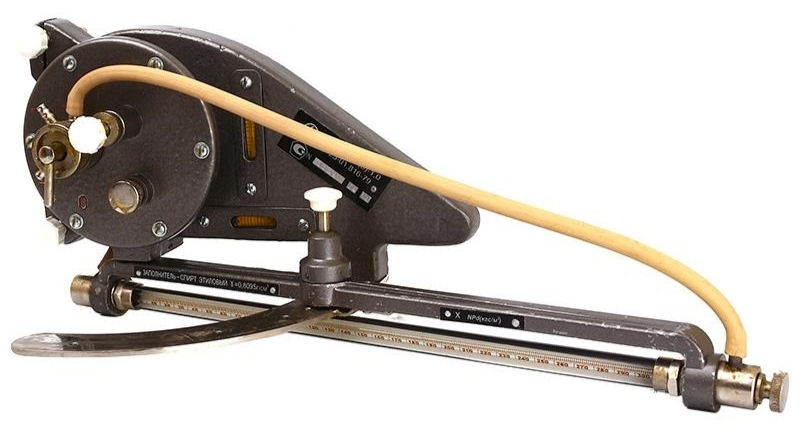
\includegraphics[scale=0.3]{Images_viscosty/manometer.jpg}
        \caption{Микроманометр}
        \label{fig:my_label}
    \end{figure}
\end{frame} 
\begin{frame}{Установка: полная схема}
    Полная установка состоит из микроманометра, газового счетчика и трубок разного диметра для измерения параметров проходящего воздуха.
    \begin{figure}
        \centering
        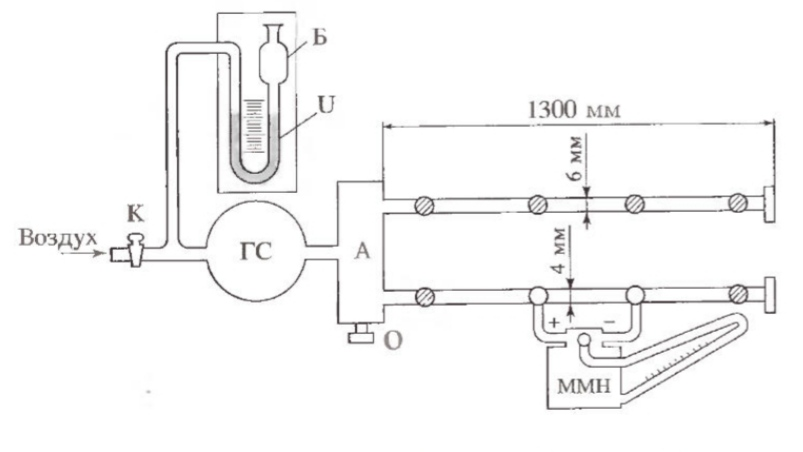
\includegraphics[scale=0.3]{Images_viscosty/full.jpg}
        \caption{Установка}
        \label{fig:my_label}
    \end{figure}
\end{frame}

\begin{frame}{Внешние условия в ходе эксперимента}
\begin{block}{Температура }
21.6 C
\end{block}
\begin{block}{Влажность }
22 \%
\end{block}
\begin{block}{Давление }
974.4 торр
\end{block}
Табличное значение вязкости воздуха при \(22^{\circ}C\) - \(1,82\cdot10^{-5}\)Па.
\end{frame}

\begin{frame}{Теоретические сведения}
    Одной из главных характеристик движения газа в трубе являеться число Рейнольдса \[Re = \frac{E_{\text{кин}}}{A_{\text{вяз}}} \equiv  \frac{v r\rho}{\eta} \]
    Ламинарное течение устанавливается на длине \textbf{a} \[\textbf{a} \approx 0,2rRe\]
    Расход воздуха при ламинарном течении в соответствии с формулой Пуазейль
    $$Q = \frac{\pi r^4}{8l\eta}\Delta P$$
\end{frame}
\begin{frame}{Предварительные оценки}
Исходя из представленной модели проведем предварительные оценки: 
$$ Q_{криит} = u \cdot \pi \cdot r^2$$
$$ Re  = \frac{\rho u R}{\eta} \Rightarrow  Q = \frac{Re \cdot \eta}{\rho} \cdot r \pi \ \propto \ 2.16 \cdot 10^{-4} $$
$$ Q = \frac{\pi R^4 \Delta P}{8 \eta l} \Rightarrow \Delta P = \frac{Re \cdot \eta}{\rho r} \cdot r^2 \pi \  \cdot \frac{8 \eta l}{\pi r^4} = \frac{Re \cdot 8 \eta^2 l}{\rho \cdot r^3} = 4.68 \cdot 10^{1} \ Па$$ 
$$ l = 0.2 \cdot r \cdot Re = 0.82 \ \text{м}$$
    
\end{frame}

\begin{frame}{Результаты измерений: \(Q \text{ от } \Delta P\)}
\begin{minipage}{.5\textwidth}
\begin{figure}
    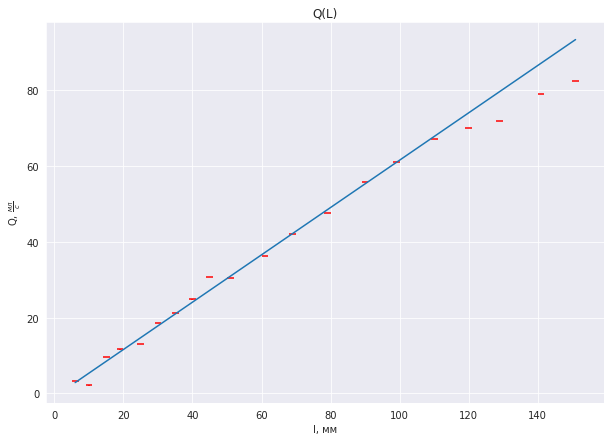
\includegraphics[scale=0.3]{Images_viscosty/First.png}
    \caption{d = 4.1 мм, k_{\text{наклона}} = 0.62}
    \label{fig:my_label}
\end{figure}
\end{minipage}%
\begin{minipage}{.5\textwidth}
\begin{figure}
    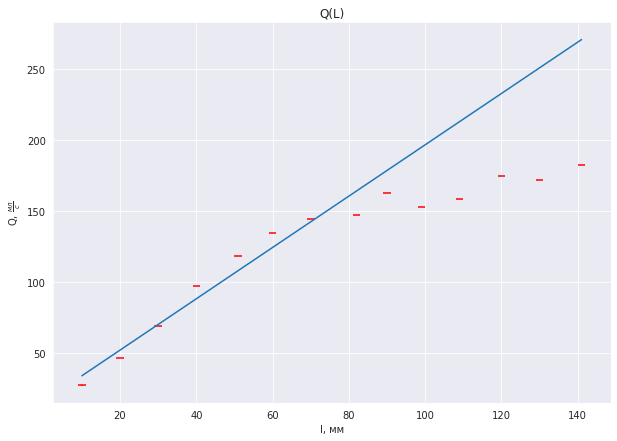
\includegraphics[scale=0.3]{Images_viscosty/Second.png}
    \caption{d = 5.2 мм, k_{\text{наклона}} = 1.80 }
    \label{fig:my_label}
\end{figure}
\end{minipage}%
    \\
    На графиках представлены результаты измерений расхода воздуха от перепада давлений
\end{frame}
\begin{frame}{Определение вязкости воздуха}
    Будем брать данные только с линейного участка, т.к он характеризуется ламинарным течением. \\
    Показание манометра в Паскали переводятся формулой \[P = 9,81 \cdot K \cdot l\] \( \K\) - коэффициэнт наклона манометра, \(l\) - его показания \\
    \\ 
    Полученные значения вязкости \(\eta_1 = (2,06\pm 0,14)\cdot10^{-5}\)Па/с, \(\eta_2 = (2,14\pm 0,15)\cdot10^{-5}\)Па/с совпадают в пределах погрешости.\\

\end{frame}
\begin{frame}{Результаты измерений: \(\Delta P \text{ от } l\)}
    Перепад давлений на разных длинах трубок радиусов 3 и 5.2 мм: 
    \begin{figure}
    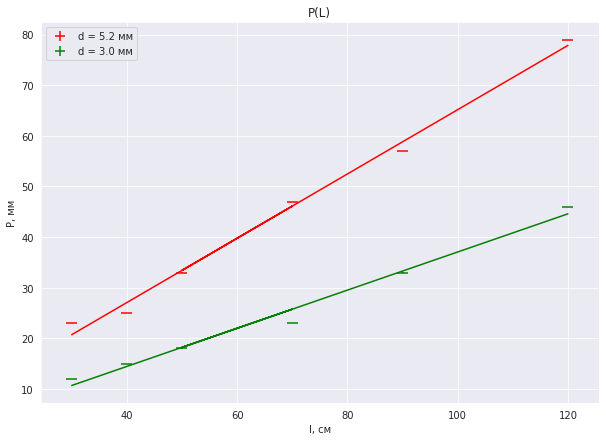
\includegraphics[scale=0.40]{Images_viscosty/p_l.png}
    \caption{k_{\text{green}} = 0.38, k_{\text{red}} = 0.63}
    \label{fig:my_label}
\end{figure}
\end{frame}
\begin{frame}{Проверка формулы Пуазейля}
  Построим график \(ln(\frac{8Ql\eta}{\pi \Delta P}) \text{ от } ln(r)\) на ламинарном участке, его коэффициэнт наклона - это показатель степени в формуле Пуазейля. Который согласно теории должен был быть равен 4. на трубке с радиусом \(3,00\pm0,05\) \ мм взята точка. \(\Delta P = 60 \pm 1 мм, \(Q = 10,8 \pm \ 0,2 \)мл/с. Коэффициэнт наклона \(k = 4,17\)
    \begin{figure}
        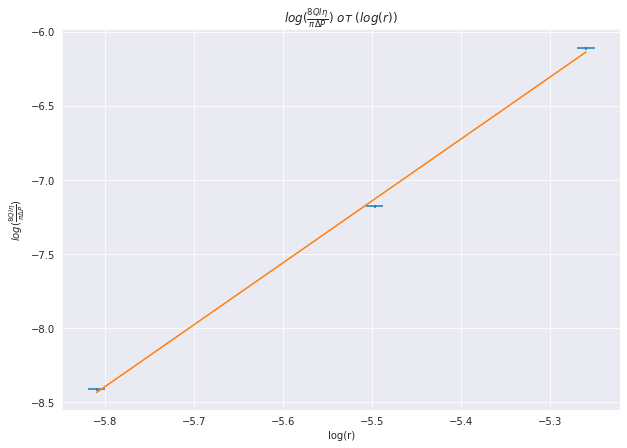
\includegraphics[scale=0.35]{Images_viscosty/last.png}
        %\caption{d = 5.2 мм, k_{\text{наклона}} = 1.80 }
        \label{fig:my_label}
    \end{figure}
  
\end{frame}
\begin{frame}{Вывод}
\begin{itemize}
    \item   В ходе работы было иследовано устанавление течений потока воздуха: $l_{\text{турбо}} = (92 \pm 3)$ см и оценка для ламинарного течения 82 см
    \item  Получена вязкость воздуха на 2 разных трубках:
    $$ \(\eta_1 = (2,06\pm 0,14)\cdot10^{-5}\) \text{Па/с},\  \(\eta_2 = (2,14\pm 0,15)\cdot10^{-5}\)\text{Па/с} $$
    Значения равны в пределах погрешности, и совпадают с табличным \(1,82\cdot10^{-5}\)Па с точностью до 14\%
    
    \item     Показатель степени в формуле Пуазейля равен 4.17, что совпадает с 4 с точностью 4\%. На 3х предоставленных точках наблюдаеться режим тока, который можно считать Пуазейлевским, но данных не достаточно много для построения гипотезы
\end{itemize}
\end{frame}

\begin{frame}{Использованные источники}
    \begin{enumerate}
        \item \href{https://www.dokipedia.ru/document/5319908?pid=150}{Таблица вязкости воздуха от макро параметров}
        \item \href{https://mipt.ru/education/chair/physics/S_II/lab/133.pdf}{Лабораторная работа 1.3.3}
        \item Кириченко - Термодинамика
        \item \href{https://docs.google.com/spreadsheets/d/16-xvHyhHE6TZBMZQnDGtpvOyMQLfq6wyw0M_AGe8FYA/edit?usp=sharing}{Таблица с данными}
    \end{enumerate}
\end{frame}

\begin{frame}{Аппендикс 1.}
\begin{minipage}{.5\textwidth}
\begin{figure}
    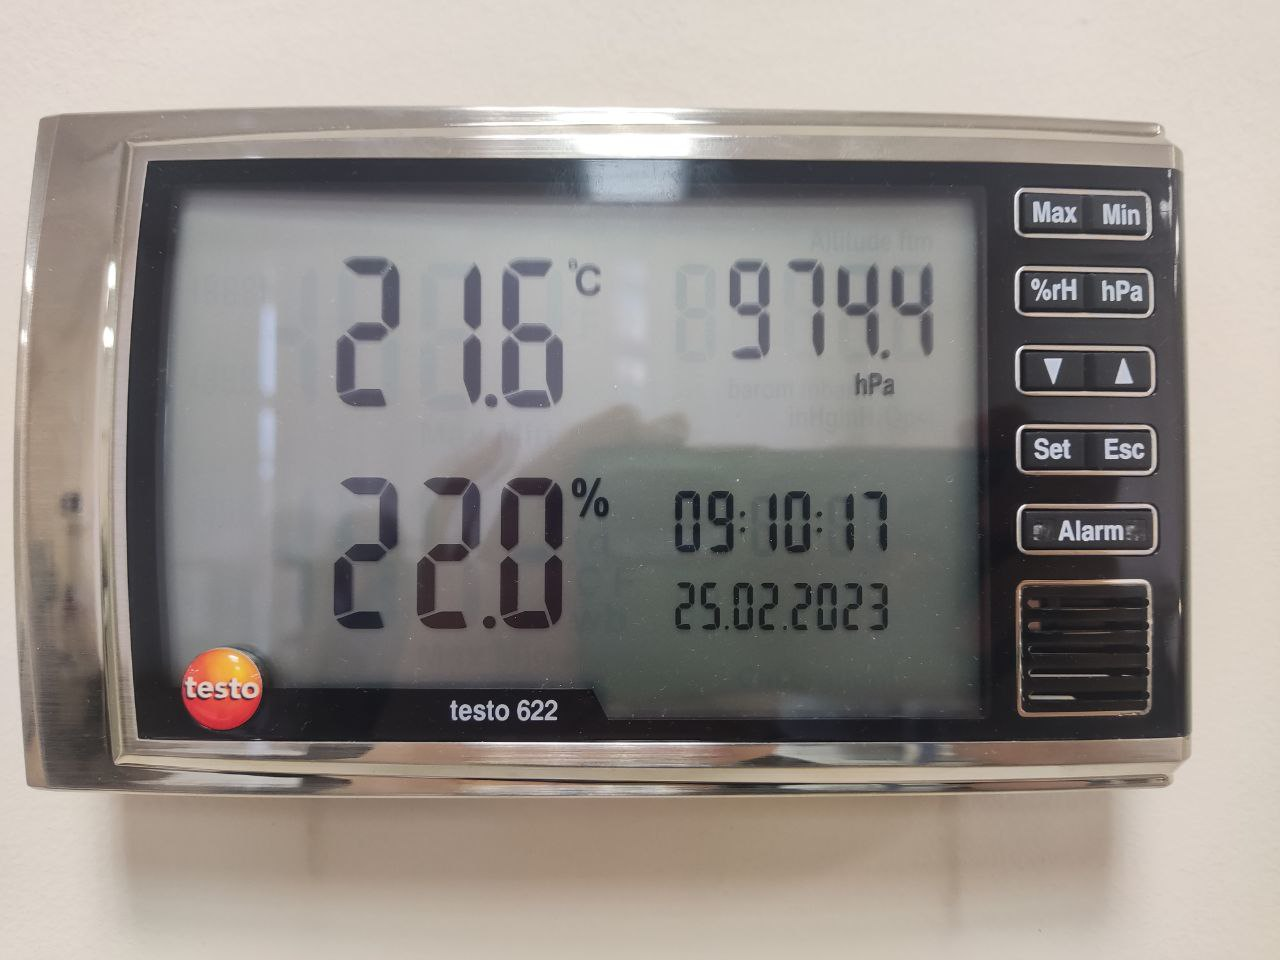
\includegraphics[scale=0.15]{Images_viscosty/photo_2023-03-11_09-20-17.jpg}
\end{figure}
\end{minipage}%
\begin{minipage}{.5\textwidth}
\begin{figure}
    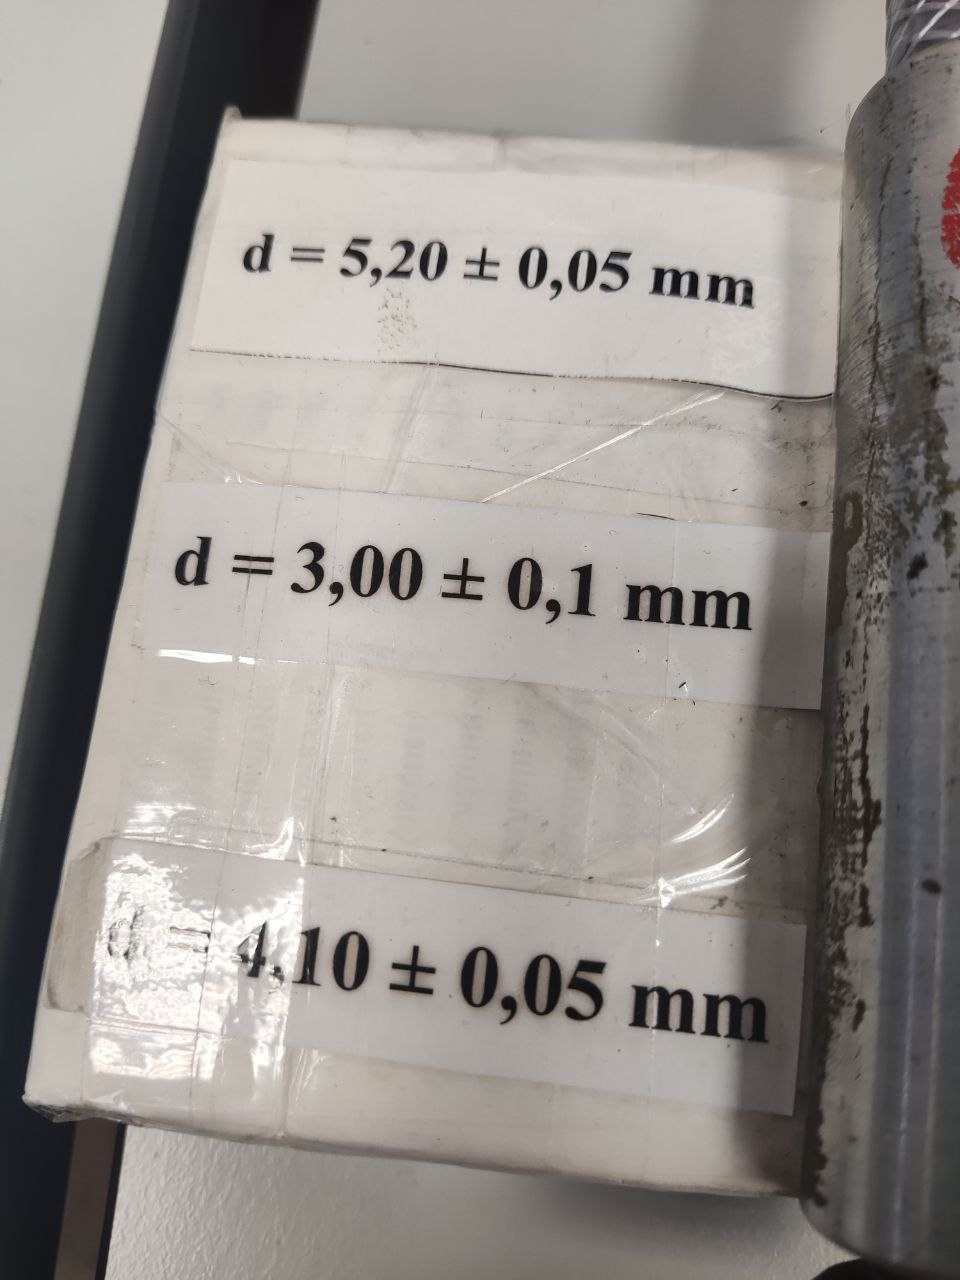
\includegraphics[scale=0.12]{Images_viscosty/lengths.jpg}
\end{figure}
\end{minipage}%
\end{frame}



\begin{frame}{Аппендикс 2.}
\begin{figure}
    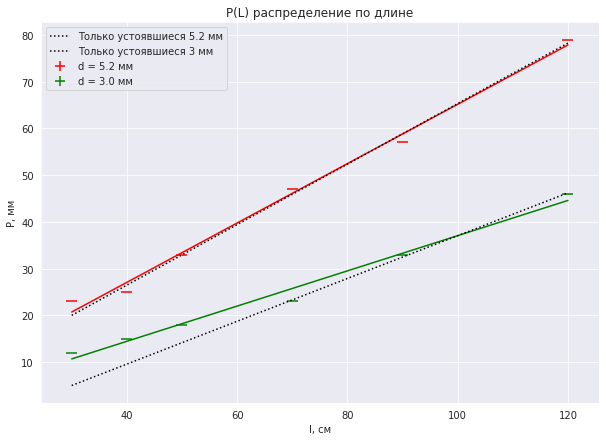
\includegraphics[scale=0.40]{Images_viscosty/asAlways.png}
    \caption{Данные слегка не сходятся}
    \label{fig:my_label}
\end{figure}
\end{frame}